\documentclass[a4paper,10pt]{article}
\usepackage{graphicx}
\usepackage{float}

%opening
\title{Assingment 2: Differentiation and Integration}
\author{Jan Laan (5756529) \\ Joost Hekman (5887232)}

\begin{document}

\maketitle


\section{Differentiation}

\subsection{Assignment 1: Calculate derivatives}
  \subsubsection{Experiment}
  Write a set of routines to perform numerical differentiation on a given function, given a parameter value
  $x$ and an increment h. Use right-hand and central differencing.
  Now use these routines to find the derivative of $\sin(x)$ for $x = \pi/3, 100\pi + \pi/3, 10^{12} \pi + \pi/3$. Experiment with the value of h to find the most accurate result in each case.
  For what value of h do you find the most accurate result in each case and what is that result.
  
  \subsubsection{Results}

  We performed the experiments found in the previous section. Results are shown below
  \textit{Note: } The correct result is always exactly $\frac{1}{2}$.
  
  \begin{figure}[H]
 
    \begin{tabular}{|c|c|c|c|c|}
      \hline
      \textbf{$\sin(x)$} & h=0.1 & h=0.01 & h=0.001 & h=0.0001\\
      \hline
      \hline
      $\pi/3$ & 0.523432 & 0.504322 & 0.500433 & 0.500043\\
      \hline
      $100\pi + \pi/3$ & 0.542432 & 0.504322 & 0.500433 & 0.500043\\
      \hline
      $10^{12} \pi + \pi/3$ & 0.543090 & 0.492491 & 0.488782 & 0.000000\\
      \hline
    \end{tabular}
    \caption{Right-hand differentiation. The value shown is the result of the calculation.}
  \end{figure}
  

  \begin{figure}[H]
 
    \begin{tabular}{|c|c|c|c|c|}
      \hline
      \textbf{$\sin(x)$} & h=0.1 & h=0.01 & h=0.001 & h=0.0001\\
      \hline
      \hline
      $\pi/3$ & 0.499167 & 0.499992 & 0.500000 & 0.500000\\
      \hline
      $100\pi + \pi/3$ & 0.499167 & 0.499992 & 0.500000 & 0.500000\\
      \hline
      $10^{12} \pi + \pi/3$ & 0.499743 & 0.488361 & 0.488369 & 0.000000\\
      \hline
    \end{tabular}
    \caption{Central differentiation. The value shown is the result of the calculation.}
  \end{figure}

  \subsubsection{Conclusions}
    If we take a look at the above tables, we can observe a few things:
    \begin{itemize}
      \item The central differentiation is much more accurate, reaching 0.5 faster, with a higher value of $h$.
      \item When used with a high input number, and a low value of $h$, the functions start returning incorrect output. For example $\sin(10^{12} \pi + \pi/2)$ starts good for $h = 0.1$, but then drops in correctness and eventually even returns $0$.
      \item A lower value of $h$ is better, but if you go too low, the funciton will fail. Best use $h=0.001$ with central differentiation. That should give the best results overall. Lower values of $h$ can be used, but with caution.
    \end{itemize}

  \subsection{Assignment 2: Bisection}

  \subsubsection{Experiment}
  Use the bisection method to find a zero of the function
                                          $$f(x) = x \sin(x) - 1$$
  on $x \in [0, 2]$.
  Record how many steps you need and at what rate the error decreases.
  
  \subsubsection{Results}
  To accurately determine the zero of the above function, with an epsilon of $0.0001$, we needed 23 steps. According to this method, the zero lies between 1.114136 and 1.114197.
  
  \subsubsection{Conclusion}
  There is nothing to conclude here, other than that bisection works. There is no comparison yet.

  \subsection{Assignment 3: Bisection, Regula Falsi and Newton-Raphson}

  \subsubsection{Experiment}
                        
  Calculate the value of $\sqrt 2$ using the bisection method.
  Record how many steps you need and at what rate the error decreases. Now do the same experiment
  using the ``false position'' method and Newton-Raphson.
  
  \subsubsection{Results}
  All three methods managed to find the result of $\sqrt 2$. This is their performance:
  \begin{itemize}
    \item Bisection: 25 steps.
    \item Newton-Raphson: 4 steps. (Using a guess of 4,5)
    \item Regula Falsi: 23 steps.
  \end{itemize}
  
  \subsubsection{Conclusion}
  As we can see, the Newton-Raphson approach is vastly superior to the other two. However, this method depends on a decent initial guess of the outcome. If the guess is really wrong, it will take longer with this method. It would be better to perform a few iterations of Regula Falsi, and then use the Newton-Raphson method with the result of that. This should always give the result in a low amount of steps.


  \subsection{Assignment 4: More Newton Raphson}

  \subsubsection{Experiment}

    Use the Newton-Raphson method to compute the zeros of
                                              $$f(x) = x2 - x + 2$$
    and
                                            $$f(x) = x3 - 3x - 2$$
    and
                                          $$f(x) = (x2 + 1)(x - 4)$$
    How do you find a suitable starting value for x? Would it help to do the first few iterations using the
    bisection or regula falsi methods?


    At first, we simply ``guessed'' the result of the functions. The results of this were just down to the accuracy of our guesses of course. That is not an accurate way of going about it. So we implemented the following: First perform steps with the Regula Falsi method to determine a base guess (Untill you've determined the value up to a range of 10), then switch to Newton-Raphson.
  
  \subsubsection{Results}
  For these functions, the results are as follows:

  \begin{tabular}{|c|c|c|}
    \hline
    Function & \# Regula Falsi steps & \# Newton-Raphson steps\\
    \hline
    $f(x) = x2 - x + 2$ & 3 & n/a\\
    $f(x) = x3 - 3x - 2$ & 56 & 0\\
    $f(x) = (x2 + 1)(x - 4)$ & 59 & 0\\
    \hline
  \end{tabular}

  \subsubsection{Conclusion}

  As you can see, in two of our three examples the regula falsi already very accurately approached the final result, so the Newton Raphson method had no work left to do. This is because the RF method first worked out oue part of the function (f.e.: The part below zero), almost to completion, and only then decimated the other half, immediately jumping from a large difference between the two bounds to a very small one. Unfortunately this doesn't help us at all in drawing conclusions. For other functions this combined method should be more succesfull hopefully.
  
\section{Integration}

  \subsection{Assignment 5: Integration}

  \subsubsection{Experiment}
  Write three routines to integrate a function over a specified interval, one using the rectangle rule, one
  using the trapezoidal rule, the third using Simpson and finally one using a two-point Gauss integration.
  All four should allow you to specify how many subdivisions should be used on the interval.
  Test the accuracy of those routines for the following integrals:
  $$\int_0^1 \! e^{-x} \, \mathrm{d}x$$
  $$\int_0^2 \! xe^{-x} \, \mathrm{d}x$$
  $$\int_0^{20} \! xe^{-x} \, \mathrm{d}x$$
  $$\int_0^{200} \! xe^{-x} \, \mathrm{d}x$$
  $$\int_0^{8\pi} \! \sin(x) \, \mathrm{d}x$$
Can you also calculate the following integral (you should be able to do it by hand):
$$\int_0^2 \! x^{-0.5} \, \mathrm{d}x$$

  \subsubsection{Results}

  \begin{figure}[H]
  \begin{tabular}{|c|c|c|c|c||c|}
  \hline
  Function & TZ & RT & SI & GA & REAL\\
  \hline
  $\int_0^1 \! e^{-x} \, \mathrm{d}x$ & 0.632647 & 0.631857 & 0.632121 & 0.632116 & 0.632121\\
  $\int_0^2 \! xe^{-x} \, \mathrm{d}x$ & 0.590216 & 0.595881 & 0.593969 & 0.593991 & 0.593994\\
  $\int_0^{20} \! xe^{-x} \, \mathrm{d}x$ & 0.724062 & 1.11729 & 0.864053 & 0.999979 & 1\\
  $\int_0^{200} \! xe^{-x} \, \mathrm{d}x$ & 0.724062 & 1.11729 & 0.864053 & 0.999994 & 1\\
  $\int_0^{8\pi} \! \sin(x) \, \mathrm{d}x$ & $0.63998 * 10^{-16}$ & 0 & $1.09332 * 10^{-16}$ & $3.48787 * 10^{-16}$ & 0\\
  $\int_0^2 \! x^{-0.5} \, \mathrm{d}x$ & INF & 2.5582 & INF & 2.71111 & 2.82843\\
  \hline
  \end{tabular}
    \caption{TZ = Trapezoidal method, RT = Rectangle method, SI = Simpson method, GA = Gauss method, REAL = Intended result (Acorrding to Wolfram Alpha)}
  \end{figure}
  
  \subsubsection{Conclusion}
  If we look at the table,w e can see that the Gaussian method is the most accurate one, followed by the Simpson method and the Trapezoidal method. The rectangle method is trailing at the bottom of the pack.

  With the last integral we see that the Gaussian and the Rectangle method are the more robust ones. They still produce an answer, while the Trapezoidal and Simpson methods simply return INF.

  \subsection{Assignment 6: Nummerical integration: Accuracy}

  \subsubsection{Experiment}
  Now try to create a routine that integrates a function with a desired
  accuracy, by computing the integral with different numbers of sample
  points, comparing the results and increasing the number of sample points
  if the required accuracy is not attained. Think carefully about how
  you should define the accuracy. Do this for each of of the above four
  methods and investigate how many refinements you need for each to reach
  a specified accuracy. Test your routines on some suitably challenging integrals.

  \subsubsection{Results}
  To determine the best possible accuracy of an integral, you have to
  have some boundry, lets call it epsilon. Then you can integrate on
  some starting number of subdivisions, say 1. Then a second time for
  comperision, with a fixed added number so say 1 again. Then you have
  an interation of 1 and 2 subdivisions. Now, if there is any difference
  between the two that is greater then epsilon, you will have to compute
  another integral with 2 plus 1 subdivisons. Again, you have to compare
  the last two integrals and see if there is any difference between the
  two smaller than epsilon, and so on. If you find no difference between
  two iterations of subdivisions of integrals, you have found the
  maximal accuracy.\\

  Here are the results for the following formula: $$\int_0^4 \! \frac{x^{\frac{5}{6}} (4 -
  x)^{\frac{1}{6}}}{(5 - x)(6 - x)(7 - x)} \, \mathrm{d}x$$ \emph{Note:} The correct
  answer is 0.284205

  \begin{figure}[H]
    \begin{tabular}{|c||c|c|c|}
    \hline
    Integration type & Calculated value & Accuracy (epsilon) & Number of
    steps taken from 1 \\
    \hline \hline
    Trapezoid & 0.283669 & 0.000001 & 628 \\
    Rectangle & 0.286869 & 0.000001 & 13 \\
    Simpson & 0.145542 & 0.000001 & 5 \\
    Gauss & 0.290936 & 0.000001 & 4 \\
    \hline
    \end{tabular}
    \caption{Best results using the maximum accuracy}
  \end{figure}

  \subsubsection{Conclusion}
  As we can see, as long as you make your accuracy very high, i.e.: your
  epsilon very small, even the two crudest implementations get the right
  answer. However, greater accuracy doesn't mean that the two finer
  implementations get the right answer. Simpsons method doesn't even
  get close. Improving the accuracy didn't help here, except for
  prolonging the execution time by a fair bit, so we can conclude here
  that although the finest implementations do help with smaller
  epsilons, larger epsilons do improve the crude implementations.

  Ofcourse, the execution time of the crude methods is far higher than
  that of the more sophisticated ones.

  \subsection{Assignment 7: Fibonacci \& Rabbit populations}

  \subsubsection{Experiments}
  The Fibonacci sequence was derived for a population of rabbits, counting
  pairs of rabbits. If you start with a single pair, it takes a month for
  that pair to reach maturity, and after that, every month they give birth
  to another pair of rabbits. These reach maturity in a month, etc. etc.
  Rabbits are assumed to live forever, generating new offspring every month.
  Most assumptions above are disputable, the one that rabbits live forever
  most clearly so. Write a program that can generate the Fibonacci sequence
  from the above assumptions, but also similar sequences where it is assumed
  that a rabbit lives only a predetermined number of months. Use this 
  program to generate such sequences and investigate how the maximum age
  affects the growth rate.
  For the original Fibonacci sequence the number of rabbits in the first 
  generation is constant (1 pair), for the second generation (the children
  of the original pair) it increases linearly in time after some point. What
  can you say about the number of rabbits in generation \emph{n}?

  \subsubsection{Results}
  We implemented Fibonacci using arrays with the first and second index hard
  coded to 0 and 1 respectively and let the following occurences be
  determined by recursive calls to n-1 and n-2. For the implementation of
  Fibonacci with limited lifespan of each rabbit generation, we added a test
  to see if n-g is larger then 0, where g is the lifespan of the
  generations. If it is, we add a recursive call for n-g, otherwise we add
  nothing (0).

  We plotted both the Fibonacci without limited lifespan as the one with
  limit lifespan set to 4 months. For the number of generations we choose
  69.

  \begin{figure}[H]
    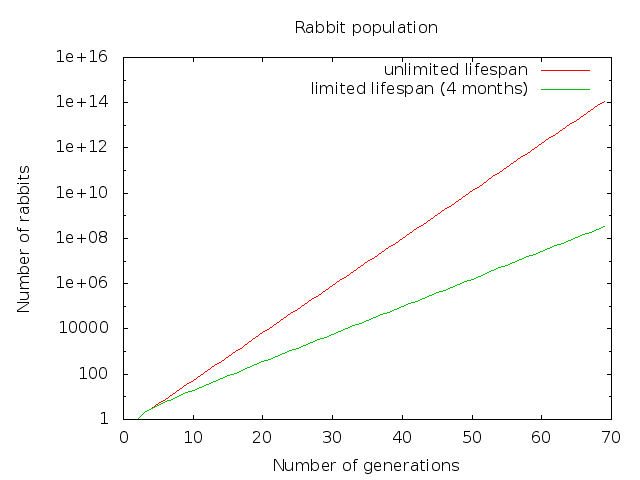
\includegraphics[scale=0.5]{plot.png}
    \caption{Rabbit population according to Fibonacci.}
  \end{figure}

  \subsubsection{Conclusion}
  The results of both growth rates of the population of rabbits with or
  without a limited lifespan show us this:
  
  \begin{itemize}
    \item Both growth rates are exponential.
    \item The difference between the two grows linearly.
  \end{itemize}

  This leaves us with the conclusion that you can say about the number of
  rabbits \emph{r} in generation \emph{n} that it equals some function of the form:

  $$ r = c * \mathrm{e}^ {(n * d) + f} + e$$

  Where \emph{c}, \emph{d}, \emph{e} and \emph{f} equal a constant number.

\end{document}
